\documentclass{article}
\usepackage{scriptStyle}
\hfuzz=1000pt
\hbadness=10000

\begin{document}

\begin{titlepage}
    \centering
    \vspace*{3cm}
    \Large\textbf{Wahrscheinlichkeitstheorie und Mathematische Statistik}

    \vspace{1cm}
    \large
    Prof.\ Dr.\ rer.\ nat.\ Martin\ Redmann\\
    Sommersemester 2025

    \vfill
\end{titlepage}

\tableofcontents
\markboth{}{}
\newpage
\vspace*{2cm}
\begin{center}
    \begin{minipage}{0.85\textwidth}
        \small
        Diese Mitschrift basiert auf der gleichnamigen Vorlesung \textit{Wahrscheinlichkeitstheorie und 
        Mathematische Statistik}, gehalten im Sommersemester 2025 
        an der Universität Rostock.\\[0.5em]
        Alle Rechte an Inhalt und Struktur der Lehrveranstaltung liegen bei dem Modulverantwortlichen, 
        Prof.\ Dr.\ rer.\ nat.\ Martin\ Redmann, sowie der Universität Rostock.\\[0.5em]
        Diese Mitschrift dient ausschließlich zu Lern- und Dokumentationszwecken. Eine kommerzielle Nutzung oder 
        Weiterverbreitung ohne Zustimmung ist nicht gestattet.
    \end{minipage}
\end{center}


% !TeX root = ../script.tex

\newpage
\section{Einleitung}

% !TeX root = ../script.tex

\newpage
\section{Ergänzugen/Wiederholung Wahrscheinlichkeitstheorie}

\subsection{Gesetz der großen Zahlen}
\begin{colbox}{Lemma}[Ungleichung von Markov]\label{lem:markovUng}\ \\
    Es sei $X$ eine integrierbare Zufallsgröße, d.\,h. $\E|X|<\infty$, dann gilt für alle $\epsilon>0$:
    \[
    \P\big(\{\omega:|X(\omega)|\geq\epsilon\}\big) \leq \frac{1}{\epsilon}\E|X|
    \]
\end{colbox}
\textit{Beweis.} \\
Verwenden wir die Definition des Erwartungswertes mittels Stieltjes-Integral so ergibt sich die Ungleichung durch 
Anwendung der Linearität und Montonie des Integrals:
\begin{align*}
    \E|X| &= \int_{\R} |x| \, \diff F_X(x) \\
    &= \underbrace{\int_{\{x:|x|<\epsilon\}} |x| \, \diff F_X(x)}_{\geq 0} + 
    \int_{\{x:|x|\geq\epsilon\}} |x| \, \diff F_X(x) \\
    &\geq \int_{\{x:|x|\geq\epsilon\}} |x| \, \diff F_X(x) \\
    &\geq \int_{\{x:|x|\geq\epsilon\}} \epsilon \, \diff F_X(x) \\
    &= \epsilon\cdot \int_{\{x:|x|\geq\epsilon\}} \diff \mu_X(x) \\
    &= \epsilon\cdot\mu_X\big(\{x:|x|\geq\epsilon\}\big) \\
    &= \epsilon\cdot \P\Big(\big\{\omega:X(\omega)\in\{x:|x|\geq\epsilon\}\big\}\Big) \\
    &= \epsilon\cdot \P\big(\{\omega:|X(\omega)|\geq\epsilon\}\big) 
\end{align*}
\qed 
\begin{colbox}{Bemerkung}
    Aus Lemma~\ref{lem:markovUng} folgt
    \begin{align*}
        \P(|X-\E[X]|\geq\epsilon) &= \P\big( \underbrace{|X-\E[X]|^2}_{\text{neue Zufallsgröße}}\geq\epsilon^2\big) \\
        &\leq \frac{1}{\epsilon^2}\E|X-\E[X]|^2 \\
        &= \frac{1}{\epsilon^2} D^2[X]
    \end{align*}
\end{colbox}
Analog lässt sich auch die \emph{Tschebyscheffsche Ungleichung} herleiten, für ein beliebiges $p>0$ gilt
\[\P(|X|\geq\epsilon) \leq \frac{E|X|^p}{\varepsilon^p}\]

\begin{colbox}{Definition}[Fast sichere Konvergenz]
    Gegeben sei ein Wahrscheinlichkeitsraum $(\Omega, \mathcal{F}, \P)$. Eine Folge $(X_n)$ von Zufallsgrößen 
    konvergiert fast sicher gegen eine Zufallsgröße $X$, falls eine Nullmenge $N\in\mathcal{F}$, d.h. $\P(N)=0$, 
    existiert, so dass 
    \[
        \lim_{n\to\infty} d(X_n(\omega), X(\omega)) = 0 \qquad \text{für alle }\omega \in \Omega\backslash N
    \]
    äquivalent dazu konvergiert eine Folge reeller Zufallsgrößen fast sicher, wenn 
    \[
        \P\Big(\Big\{\omega\in\Omega\,\Big|\,\lim_{n\to\infty} X_n(\omega)= X(\omega) \Big\}\Big) = 1
    \] 
\end{colbox}

\begin{colbox}{Definition}[Stochastische Konvergenz]\ \\
    Eine Folge $(X_n)$ von Zufallsgrößen \emph{konvergiert stochastisch} (oder in Wahrscheinlichkeit) gegen eine 
    Zufallsgröße $X$, falls
    \[
    \P\big(\{\omega:|X_n(\omega)-X(\omega)|>\epsilon\}\big) 
    \xrightarrow{n\to\infty} 0\quad\text{für alle }\epsilon \geq 0
    \]
    oder dazu äquivalent, falls
    \[
    \P\big(\{\omega:|X_n(\omega)-X(\omega)|\leq\epsilon\}\big) 
    \xrightarrow{n\to\infty} 1\quad\text{für alle } \epsilon > 0
    \]
    Wir schreiben im folgenden auch $X_n\conP X$ mit $n\to\infty$ oder sagen, dass $X_n$ mit Wkt. 1 konvergiert.
\end{colbox}
\begin{colbox}{Definition}[Definition des schwachen Gesetzes der großen Zahlen]\label{def:schwachesGesetz}\ \\
    Eine Folge integrierbarer Zufallsgrößen $(X_n)$, d.\,h. $\E|X_n|<\infty\ \forall\,n$ genügt genau dann
    dem schwachen Gesetz der großen Zahlen, wenn
    \[
    \frac{1}{n}\sum_{k=1}^{n}(X_k-\E[X_k]) \conP 0,\quad\text{für }n\to\infty.
    \]
\end{colbox}
Ein Spezialfall bilden hier Beobachtungen: Seien $X_1,\dotsc,X_n$ unabhängige Beobachtungen einer Zufallsgröße $X$, 
so gilt $\E[X_k]=\E[X]$ und der Term vereinfacht sich durch
\[
\frac{1}{n}\sum_{k=1}^{n}(X_k-\E[X_k]) = \frac{1}{n}\sum_{k=1}^{n}X_k-\E[X]
\]
\begin{colbox}{Satz}[Schwaches Gesetz der großen Zahlen, $L^1(\Omega,\mathcal{F},\P)$ Version]\ \\
    Es sei $(X_n)$ eine Folge von Zufallsgrößen $X_n$, welche unabhängig und gleichverteilt wie eine integrierbare
    Zufallsgröße $X$ sind. 
    Dann genügt $(X_n)$ dem schwachen Gesetz der großen Zahlen (gemäß Definition~\ref{def:schwachesGesetz}), 
    d.\,h. konkret, dass
    \[
    \frac{1}{n}\sum_{k=1}^{n} X_k \conP \E[X], \quad \text{für } n \to \infty.
    \]
\end{colbox}
\textit{Ohne Beweis.}\\

% Wir schreiben $X_k = X_k^+ - X_k^-$, wobei $X_k^+$ und $X_k^-$ jeweils den Positiv- und Negativteil von $X$ enthalten, 
% d.h. 

% \[
%     X_k^+ := \max\{X_k, 0\}, \qquad X_k^- := \max\{-X_k, 0\}
% \]

% Demnach gilt: 

% \[
%     \dfrac{1}{n}\sum_{k=1}^{n} (X_k - \E[X_k]) 
%     = \underbrace{\dfrac{1}{n}\sum_{k=1}^{n} (X_k^+ - \E[X_k^+])}_{=:S_n^+} 
%     - \underbrace{\dfrac{1}{n}\sum_{k=1}^{n} (X_k^- - \E[X_k^-])}_{=:S_n^+} 
% \]

% Es genügt nun zu zeigen, dass die einzelnen Summanden $S_n^+$ und $S_n^-$ gegen 0 mit Wkt. 1 konvergieren, damit auch 
% ihre Differenz es tut. Wir können also o.B.d.A. annehmen, dass $X_i\geq 0$.

% Wir definieren eine neue Zufallsgröße

% \[
%     \tilde{X}_i := X_i\cdot \One_{\{X_i\leq i\}}
% \]

% Nun gilt 

% \begin{align*}
%     \sum_{n=1}^{\infty} \P(X_n \neq \tilde{X}_n) 
%     &= \sum_{n=1}^{\infty} \P(X_n > n) 
%     = \sum_{n=1}^{\infty} \P(X > n) 
%     \leq \sum_{n=1}^{\infty} \P(X \geq n) \\
%     &= \sum_{n=1}^{\infty} \P(X \geq n) 
%     = \sum_{n=1}^{\infty}\sum_{k=n}^{\infty} \P(k+1 > X \geq k)
%     = \sum_{k=1}^{\infty}\sum_{n=1}^{k} \P(k+1 > X \geq k)\\
%     &= \sum_{k=1}^{\infty}k \cdot \P(k+1 > X \geq k)
%     = \E\left[\sum_{k=1}^{\infty}k \cdot \P(k+1 > X \geq k)\right]\\
%     &\leq \E\left[\sum_{k=1}^{\infty}X \cdot \P(k+1 > X \geq k)\right]
%     = \E[X] < \infty
% \end{align*}

% Das Lemma von Borel-Cantelli garantiert damit also, dass 

% \[
%     \P\big(\liminf_{n\to\infty} (X_n \neq \tilde{X}_n)^C\big) = 1
% \]

% Für uns bedeutet dies, dass für fast alle $\omega\in\Omega$ ein $N_\omega\in\N$ existiert, sodass 
% $X_n(\omega)=\tilde{X}_n(\omega)$ für alle $n\geq N_\omega$ gilt. Is also $n$ hinreichend groß, dann gilt 

% \[
%     \dfrac{1}{n}\sum_{k=1}^{n} X_k(\omega) - \dfrac{1}{n}\sum_{k=1}^{n} \tilde{X}_k(\omega) 
%     = \dfrac{1}{n} \sum_{k=1}^{N_\omega-1} (X_k(\omega)-\tilde{X}_k(\omega))
% \]

% Da die Summe auf der rechten Seite für ein festes $\omega$ beschränkt sein muss, konvergiert der Term gegen 0 für 
% $n\to \infty$, d.h. $\tfrac{1}{n}\sum_{k=1}^{n} X_k$ hat den gleichen Grenzwert wie 
% $\tfrac{1}{n}\sum_{k=1}^{n} \tilde{X}_k$. Es genügt also zu zeigen, dass $\tfrac{1}{n}\sum_{k=1}^{n} \tilde{X}_k$ 
% gegen $\E X$ mit Wkt. 1 konvergiert.

% Sei hierfür $\varepsilon>0$. Wir definieren $k_n := \lfloor(1+\varepsilon)^n\rfloor$. Wir beginnen zunächst damit 
% zu zeigen, dass $\tfrac{1}{k_n}\sum_{k=1}^{k_n} \tilde{X}_k$ mit Wkt. 1 gegen  $\E X$ konvergiert (d.h. wir beschränken 
% uns erst auf die Betrachtung einer Teilfolge und folgern später die Konvergenz für die gesamte Folge).



\subsection{Charakteristische Funktionen}

Bisher wurden Zufallsgrößen immer entweder durch ihre Verteilungsfunktion oder ihre Verteilungsdichte charakterisiert. 
Eine weitere solche Charakterisierung bildet die charakteristische Funktion. Sie dient als wichtiges Hilfsmittel 
für Rechnungen und Beweise (zum Beispiel beim zentralen Grenzwertsatz).

\begin{colbox}{Definition}[Charakteristische Funktion]
    Sei $X$ eine Zufallsgröße mit Verteilungsfunktion $F$, dann heißt für $t\in\R$ 
    \[
        \Psi(t) := \E[e^{itX}] = \int_{-\infty}^{\infty} e^{itx} \diff F(x)
    \]
    die charakteristische Funktion von $X$. \\ 
    
    Für die Berechnung ergeben sich zwei Fälle: \\
    Ist $X$ diskret, so gilt 
    \[
        \Psi(t) = \sum_{k} e^{itx_k}\cdot p_k, 
    \]
    wobei $(x_k)$ die Werte von $X$ mit $p_k = \P(X=x_k)$  sind.\\
    Ist $X$ absolut stetig, so gilt 
    \[
        \Psi(t) = \int_{-\infty}^{\infty}e^{itx}f(x) \diff x,
    \]
    wobei $f$ die Dichte von $X$ ist. \\ \\
    \textit{Im Fall von Zufallsvektoren $\vec{X}=(X_1,\dots,X_n)^T$ wird die charakteristische Funktion über das 
    Skalarprodukt definiert:}
    \[
    \Psi(t) := \E[e^{i\cdot\langle t,\vec{X}\rangle}] \qquad \text{mit } t = (t_1,\dots,t_n)^T
    \]
\end{colbox}

Die Eindeutigkeit der charakteristischen Funktion kommt daher, dass sie die Fouriertransformierte der Verteilung 
von $X$ ist, d.h. im absolutstetigen Fall die Transformation der Funktion $f$ und im diskreten Fall die Transformation
der Folge $p_k$. Bekannterweise ist die Fouriertransformation invertierbar und damit dient sie als Charakterisierung 
der Zufallsgröße. Diese Inverse können wir verwenden um aus bekannter charakteristischen Funktion die Dichte / 
Einzelwahrscheinlichkeiten der zugehörigen Zufallsgröße zu bestimmen:

\begin{colbox}{Satz}[Inverse der charakteristischen Funktion]
    Sei $X$ eine Zufallsgröße mit charakteristischen Funktion $\Psi$. Dann ergibt sich mittels inverser 
    Fouriertransformation :
    \begin{enumerate}
        \item[i)] 
        \[
            f(x) = \dfrac{1}{2\pi}\int_{-\infty}^{\infty}e^{-itx}\Psi(t)\diff t
        \]
        \item[ii)] 
        \[
            p_k = \lim_{T\to\infty} \dfrac{1}{2T}\int_{-T}^{T}e^{-itx_k}\Psi(t)\diff t
        \]
    \end{enumerate}
    (wieder jeweils im absolutstetigen oder diskreten Fall.)
\end{colbox}
\textit{ohne Beweis.}

Es folgen einige wichtige Eigenschaften der charakteristischen Funktion:

\begin{colbox}{Lemma}\label{lem:charEigenschaften}
    \begin{enumerate}
        \item Die charakteristische Funktion $\Psi$ ist wohldefiniert.
        \item $\Psi(0)=1$ und $|\Psi(t)|\leq 1$.
        \item $\Psi_{aX+b} = e^{itb}\cdot\Psi(at)$ für $a,b,t\in\R$.
        \item Wenn $X$ endliches $n$-tes Moment hat, dann gilt für $k=1,\dots,n$:
        \[
            \left.\dfrac{\diff^k}{\diff t^k} \Psi(t)\right|_{t=0} = i^k\cdot \E[X^k]
        \]
        \item $\Psi$ ist gleichmäßig stetig.
        \item Wenn $X$ und $Y$ unabhängig sind, dann gilt $\Psi_{X+Y} = \Psi_X\cdot\Psi_Y$
    \end{enumerate}
\end{colbox}
\textit{Beweis.}
\begin{enumerate}
    \item 
    \[
        \int_{-\infty}^{\infty} \underbrace{|e^{itx}|}_{=1} \diff F(x) 
        = \int_{-\infty}^{\infty} \diff F(x) = F(x)\Big|_\infty^\infty = 1 < \infty
    \]

    \item 
    \begin{align*}
        \Psi(0) &= \int_{-\infty}^{\infty} \underbrace{e^{i\cdot 0 \cdot x}}_{=1} \diff F(x) = 1 \\
        |\Psi(t)| &\leq \int_{-\infty}^{\infty} |e^{i\cdot t \cdot x}| \diff F(x) = 1 
    \end{align*}
    \item
    \[
        \Psi_{aX+b} = \E[\exp(it\cdot(aX+b))] = \E[\exp(itaX + itb)] = e^{itb}\cdot \E[\exp(i\cdot(at)\cdot X)] = e^{ibt}\cdot\Psi(at)
    \]
    \item 
    \[
        \left.\dfrac{\diff^k}{\diff t^k} \Psi(t) \right|_{t=0} 
        = \left.\dfrac{\diff^k}{\diff t^k} \int_{-\infty}^{\infty} e^{itx}\diff F(x) \right|_{t=0} 
        = \int_{-\infty}^{\infty} \left.\dfrac{\diff^k}{\diff t^k} e^{itx}\right|_{t=0} \diff F(x) 
        = i^k\cdot \int_{-\infty}^{\infty} x^k \diff F(x) = i^k\cdot\E[X^k]
    \]
    Das Vertauschen von Integral und Ableitung ist (nach Leibniz Regel) erlaubt, da 
    \[
        \left|\dfrac{\diff^k}{\diff t^k} e^{itx}\right| = |i^k x^k e^{itx}| = |x^k|
    \] 
    und 
    \[
        \int_{-\infty}^{\infty} |x^k| \diff F(x) = \E|X|^k < \infty
    \]
    \item Als Erinnerung: Gleichmäßig stetig heißt, dass $\sup_t|\Psi(t+h)-\Psi(t)| \to 0$ für $h\to 0$:
    \[
        |\Psi(t+h)-\Psi(t)| = \Big|\E\big[e^{i(t+h)X}\big] - \E\big[e^{itX}\big]\Big| 
        = \Big|\E\big[e^{itX}\cdot(e^{ihX}-1)\big]\Big| \leq \E\big[|e^{itX}|\cdot|e^{ihX}-1|\big] = \E|e^{ihX}-1|
    \]
    Demnach gilt für das Supremum:
    \[
        \sup_t|\Psi(t+h)-\Psi(t)| \leq \E|e^{ihX}-1| \to 0 \quad\text{für }h\to 0
    \]
    \item 
    \[
        \Psi_{X+Y}(t) = \E\big[e^{it(X+Y)}\big] = \E\big[e^{itX}\cdot e^{itY}\big] 
        = \E\big[e^{itX}\big]\cdot\E\big[e^{itX}\big] = \Psi_X(t)\cdot\Psi_Y(t)
    \]
    \qed
\end{enumerate}

\begin{colbox}{Korollar}\label{kor:charReihe}
    Aus Lemma \ref{lem:charEigenschaften} (4) ergibt sich folgende Reihenentwicklung:
    \[
        \Psi(t) = \sum_{k=0}^{\infty}\dfrac{i^k\cdot\E[X^k]}{k!}\cdot t^k
    \]
\end{colbox}

\begin{colbox}{Beispiel}[charakteristische Funktion der Poisonverteilung]
    Sei $X$ poissonverteilt mit Parameter $\lambda>0$ ($X\sim\mathrm{Poi}(\lambda)$), dann gilt:
    \begin{align*}
        \Psi(t) 
        = \E[e^{itX}] 
        = \sum_{k=0}^{\infty} e^{itk} \cdot \dfrac{\lambda^k}{k!}e^{-\lambda} 
        = e^{-\lambda}\cdot \sum_{k=0}^{\infty} \dfrac{(\lambda\cdot e^{it})^k}{k!} 
        = e^{-\lambda}\cdot e^{\lambda\cdot e^{it}} 
        = \exp\big(\lambda(1-e^{it})\big)
    \end{align*}
\end{colbox}

\begin{colbox}{Beispiel}[charakteristische Funktion der Normalverteilung]
    Sei $X\sim \mathcal{N}(\mu,\sigma^2)$ normalverteilt. Zur Bestimmung von $\Psi_X$ betrachten wir 
    $Z\sim\mathcal{N}(0,1)$, da $X = \sigma\cdot Z + \mu$. \\
    Für die Standardnormalverteilung gilt:
    \[
        \E[Z^k] = \begin{cases}
            0 & k \text{ ungerade} \\
            (k-1)!! & k \text{ gerade}\footnote{$(k-1)!!=1\cdot 3 \cdot 5\cdot \dots \cdot (k-1)$} 
        \end{cases}
    \]
    Aus Korollar \ref{kor:charReihe} folgt damit
    \begin{align*}
        \Psi_Z(t) 
        = \sum_{k=0}^{\infty}\dfrac{(it)^k\cdot\E[Z^k]}{k!} 
        = \sum_{k=0}^{\infty}(it)^{2k} \cdot \dfrac{1\cdot 3 \cdot 5\cdot \dots \cdot (2k-1)}{1\cdot2\dots (2k-1)\cdot 2k} 
        = \sum_{k=0}^{\infty} \dfrac{(it)^{2k}}{2\cdot4\dots 2k} 
    \end{align*}
    Aus $i^2=-1$ und $2\cdot4\dots 2k = 2^k\cdot k!$ ergibt sich
    \[
        \Psi_Z(t) 
        = \sum_{k=0}^{\infty} \dfrac{(it)^{2k}}{2\cdot4\dots 2k}
        = \sum_{k=0}^{\infty} \\dfrac{(-t^2\,/\,2)^k}{k!} 
        = e^{-t^2\,/\,2}
    \]
    Für $\Psi_X(t)$ ergibt sich nach Lemma \ref{lem:charEigenschaften} (3)
    \[
        \Psi_X(t) 
        = \Psi_{\sigma Z + \mu}(t) 
        = e^{it\mu}\cdot\Psi_Z(\sigma t) 
        = e^{it\mu}\cdot e^{- \tfrac{\sigma^2t^2}{2}}
    \]
\end{colbox}

\begin{colbox}{Beispiel}[Summe von Normalverteilungen]
    Es seien $X\sim\mathcal{N}(\mu_1,\sigma_1^2)$ und $Y\sim\mathcal{N}(\mu_2,\sigma_2^2)$ unabhängig. Nach Lemma
    \ref{lem:charEigenschaften} (6) gilt:
    \[
        \Psi_{X+Y}(t) 
        = \Psi_X(t)\cdot\Psi_Y(t) 
        = e^{it\mu_1}\cdot e^{- \tfrac{\sigma_1^2t^2}{2}}\cdot e^{it\mu_2}\cdot e^{- \tfrac{\sigma_2^2t^2}{2}} 
        = e^{it(\mu_1+\mu_2)}\cdot e^{- \tfrac{(\sigma_1^2+\sigma_2^2)t^2}{2}}
    \]
    Wegen der Eindeutigkeit der charakteristischen Funktion folgt daraus, dass 
    $X+Y\sim\mathcal{N}(\mu_1+\mu_2, \sigma_1^2 + \sigma_2^2)$.
\end{colbox}

\begin{colbox}{Satz}\label{satz:charKonv}
    Sei $(F_n)$ eine Folge von Verteilungsfunktionen mit zugehörigen charakteristischen Funktionen $(\Psi_n)$ und 
    sei $F$ eine Verteilungsfunktion mit charakteristischen Funktion $(\Psi)$. Dann gilt:
    \[
        F_n\to F\text{ punktweise}\footnote{an allen Stetigkeitsstellen} \iff \Psi_n\to\Psi \text{punktweise}
    \]
\end{colbox}
\textit{ohne Beweis.}

\subsection{Zentraler Grenzwertsatz und Konvergenz}

\begin{colbox}{Definition}[Konvergenz in Verteilung]
    Eine Folge von Zufallsgrößen $(X_n)$ mit Verteilungsfunktionen $(F_{X_n})$ konvergiert in Verteilung gegen eine 
    Zufallsgröße $X$, wenn 
    \[
        \lim_{n\to\infty} F_{X_n}(x) = F_X(x)
    \]
    an allen Stetigkeitsstellen der Verteilungsfunktion $F_X$ von $X$. Wir schreiben dann $X_n\conD X$.
\end{colbox}

Eine äquivalente Definition besagt, dass $X_n \conD X$ falls $\E[g(X_n)]\to \E[g(X)]$ für alle stetigen, beschränkten 
Funktionen $g$. Daraus folgt insbesondere, dass für derartige $g$ auch $g(X_n)\conD g(X)$.

\begin{colbox}{Satz}
    Wenn $X_n\conP X$, dann gilt $X_n\conD X$. \\
    Die Umkehrung gilt im Allgemeinen nicht, außer $X=c$ ist konstant.
\end{colbox}

\begin{colbox}{Definition}
    Wir führen folgende Schreibweisen ein:
    \begin{enumerate}
        \item $\displaystyle S_n := \sum_{i=1}^n X_i$
        \item $D^2[X] := \Var(X) = \E(X-\E X)^2 = \E X^2 - (\E X)^2 $
    \end{enumerate}
\end{colbox}

\begin{colbox}{Korollar}
    Für die Varianz der Summe von unabhängigen, gleichverteilten (i.i.d.) Zufallsgröße  gilt
    \[
        D^2[S_n] = D^2\left[\sum_{i=1}^{n} X_i\right] = \sum_{i=1}^{n} D^2[X_i] = n\cdot D^2[X_1]
    \]
\end{colbox}

\begin{colbox}{Satz}[Zentraler Grenzwertsatz]\label{satz:zentralerGWS}
    Sei $(X_n)$ eine Folge von i.i.d. Zufallsgrößen mit $D^2[X_1]<\infty$, so gilt 
    \[
        \dfrac{S_n-\E[S_n]}{\sqrt{D^2[S_n]}} \conD Z \sim \mathcal{N}(0,1)
    \]
\end{colbox}
\textit{Beweis.} 
Es gilt für die charakteristische Funktion von $\tfrac{S_n-\E[S_n]}{\sqrt{D^2[S_n]}}$:

\begin{align*}
    \Psi_n(t) 
    &= \E\left[\exp\left(it\cdot \dfrac{S_n-\E[S_n]}{\sqrt{D^2[S_n]}}\right)\right] \\
    &= \E\left[\exp\left(i\cdot \dfrac{t}{\sqrt{n\cdot D^2[X_1]}}\cdot\sum_{j=1}^{n}(X_j-\E[X_1])\right)\right] \\
    &= \E\left[\prod_{j=1}^{n}\exp\left(i\cdot \dfrac{t}{\sqrt{n\cdot D^2[X_1]}}\cdot(X_j-\E[X_1])\right)\right] \\
    &= \prod_{j=1}^{n}\E\left[\exp\left(i\cdot \dfrac{t}{\sqrt{n\cdot D^2[X_1]}}\cdot(X_j-\E[X_1])\right)\right]\\
    &= \E\left[\exp\left(i\cdot \dfrac{t}{\sqrt{n\cdot D^2[X_1]}}\cdot(X_1-\E[X_1])\right)\right]^n \\
    &= \Psi_Y\left(\dfrac{t}{\sqrt{n\cdot D^2[X_1]}}\right)^n
\end{align*}

wobei $Y=X_1-\E[X_1]$. 

Unter Verwendung der Taylor-Formel ergibt sich

\begin{align*}
    \Psi_Y\left(\dfrac{t}{\sqrt{n\cdot D^2[X_1]}}\right) 
    = \underbrace{\Psi_Y(0)}_{=0} + \underbrace{\Psi_Y'(0)}_{=i\E Y = 0}\cdot \dfrac{t}{\sqrt{n\cdot D^2[X_1]}} 
    + \underbrace{\Psi_Y''(0)}_{=i^2\E Y^2 = -D^2[X_1]}\cdot \dfrac{t^2}{2n\cdot D^2[X_1]} 
    + o\left(\dfrac{t^2}{n}\right) \\
    = 1 + \dfrac{-\tfrac{t^2}{2}+o(\tfrac{t^2}{n})}{n}
\end{align*}

Da $o(\tfrac{t^2}{n})\to 0$ für $n\to\infty$ folgt 

\[
    \Psi_n(t) = \left( 1 + \dfrac{-\tfrac{t^2}{2}+o(\tfrac{t^2}{n})}{n}\right)^n \to e^{-t^2\,/\,2}
\]

Dies ist genau die charakteristische Funktion der Standardnormalverteilung und damit folgt nach Satz \ref{satz:charKonv}
die Konvergenz in Verteilung gegen $\mathcal{N}(0,1)$.
\qed

\begin{colbox}{Bemerkung}
    Äquivalent umgeformt besagt der der zentrale Grenzwertsatz, dass wir Summen von i.i.d. Zufallsgrößen durch 
    eine Normalverteilung annähern können, denn Umformungen ergeben
    \[
        S_n \approx \mathcal{N}\left(\E[S_n], D^2[S_n]\right)
    \]
    und damit 
    \[
        \P(S_n \leq x) \approx \Phi\left(\dfrac{y-\E[S_m]}{\sqrt{D^2[S_n]}}\right).
    \]
\end{colbox}

\begin{colbox}{Beispiel}[Normalapproximation]
    Seien $X_1,\dots,X_n$ Bernoulli verteilt zum Parameter 1, d.h. 
    \[
        X_k := \begin{cases}
            1, \quad \text{Ereignis} A \text{trifft ein, Wahrscheinlichkeit: } p=\P(A). \\
            0, \quad \text{Ereignis} A \text{trifft nicht ein, Wahrscheinlichkeit: } 1-p=\P(A^c).
        \end{cases}
    \]
    Die Summe $S_n\sim\mathrm{Bin}(n,p)$ gibt demnach die Anzahl an Erfolgen ($A$ trifft ein) 
    nach $n$ unabhängigen Versuchen an. Dabei gilt:
    \[
        \P(S_n \leq x) = \sum_{k=0}^{\lfloor x \rfloor} \binom{n}{k}\cdot p^k\cdot(1-p)^{n-k}
    \]
    Dabei ist der Term $\binom{n}{k} = n\cdot(n-1)\dots(n-k+1)$ für große $n$ teuer zu berechnen. Nutzen wir stattdessen 
    die Annäherung durch die Standardnormalverteilung so ergibt sich:
    \[
        S_n\approx\mathcal{N}(np,np(1-p)) \implies 
        \P(S_n \leq x) 
        = \dfrac{1}{\sqrt{2\pi n^2p^2(1-p)^2}}\cdot\exp\left(-\dfrac{1}{2}\cdot\left(\dfrac{x-np}{np(1-p)}\right)^2\right)
    \]
    Bereits für das Beispiel $n=100$, $p=0.5$ ergibt sich folgender Vergleich:
    \begin{center}
        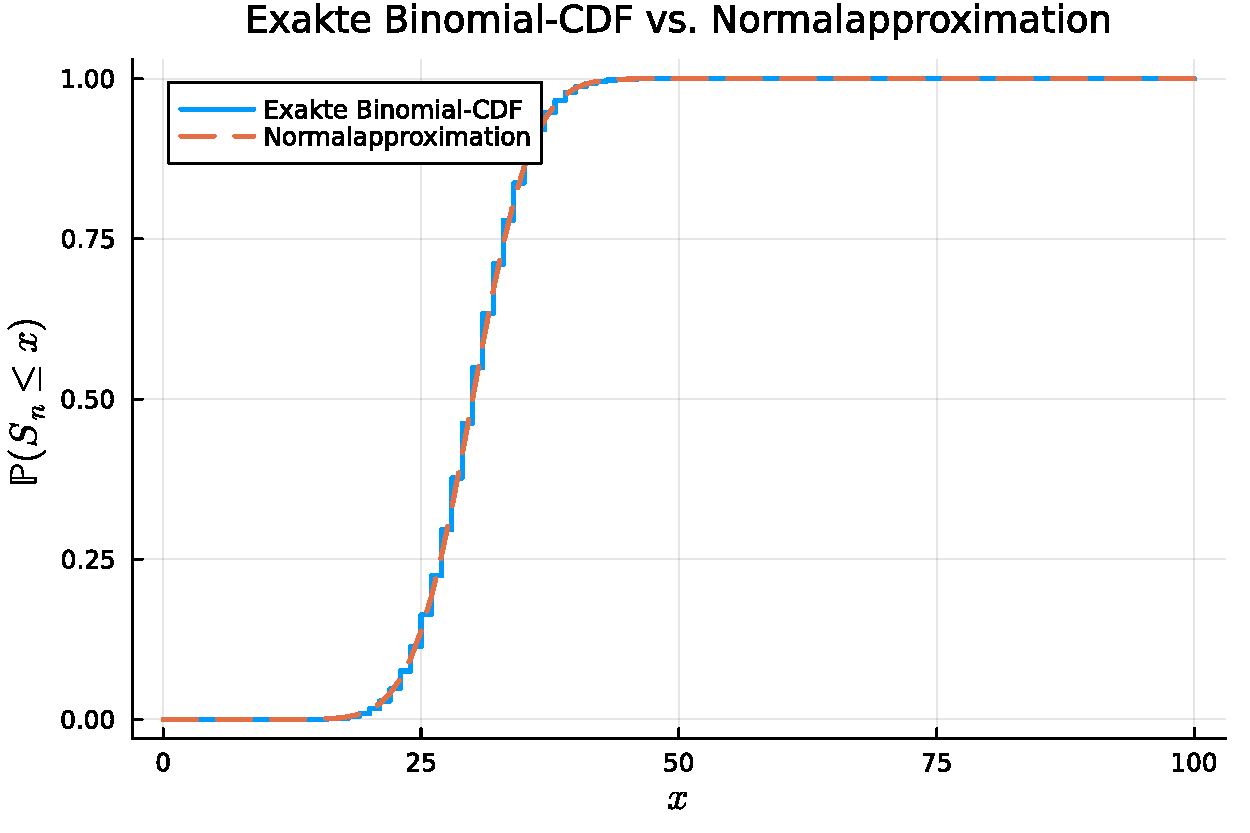
\includegraphics[width=0.8\textwidth]{images/vergleich_cdf.pdf}
    \end{center}
    mit einem maximalen quadratischen Fehler von unter 0.003.
\end{colbox}

\begin{colbox}{Beispiel}
    Als Anwendungsbeispiel betrachten wir folgenden Kontext: 

    $40\,\%$ der Menschen in Deutschland haben Blutgruppe Null. Es wird eine Stichprobe von $n=1000$ zufällig 
    ausgewählten Personen gezogen. Wie große ist die Wahrscheinlichkeit, dass zwischen $30\,\%$ bis $50\,\%$ der 
    Personen die Blutgruppe Null haben? 

    Wir definieren $Y$ als die Anzahl der Personen mit Blutgruppe Null aus den $n=1000$ zufällig befragen Personen, dann 
    ist $Y\sim\mathrm{Bin}(0.4, 1000)$. Für die Wahrscheinlichkeit, dass zwischen $38\,\%$ bis $42\,\%$ der Befragten,
    also zwischen 380 und 420 Personen, die Blutgruppe Null haben, ergibt sich
    
    \begin{align*}
        \P(380 < Y \leq 420) 
        &= \P(Y\leq 380) - \P(Y\leq 420) \\
        &\approx \Phi\left(\dfrac{420-1000\cdot0.4}{\sqrt{1000\cdot 0.4\cdot(1-0.4)}}\right)
        - \Phi\left(\dfrac{380-1000\cdot0.4}{\sqrt{1000\cdot 0.4\cdot(1-0.4)}}\right) \\
        &= \Phi\left(\dfrac{20}{\sqrt{240}}\right) - \Phi\left(-\dfrac{20}{\sqrt{240}}\right) \\
        &= 2\Phi\left(\dfrac{20}{\sqrt{240}}\right) - 1 \approx 0.803
    \end{align*}
\end{colbox}

\begin{colbox}{Beispiel}[Stichprobenumfang bei Umfragen]
    Ein unbekannter Anteil $p$ von Menschen wählt eine Partei. Dieses $p$ soll in einer Umfrage ermittelt werden.

    Gefragt ist, wie groß dem Umfang $n$ einer Stichprobe sein muss, so dass die Umfrage aussagekräftig ist.

    Dabei sei $X_1,\dots,X_n$ unsere mathematische Stichprobe (Bernoulli verteilt mit Parameter $p$). Es ergibt 
    sich dabei, dass $S_n$ die Anzahl der Wähler gesuchter Partei aus $n$ Befragten ist. 

    $S_n$ ist binomialverteilt und $\hat{p}_n = \tfrac{S_n}{n}$ ist die relative Häufigkeit des Ereignisses und dient 
    als Schätzer für den echten Anteil $p$. 

    Unser Ziel ist, dass wir mit einer Wahrscheinlichkeit von mindestens $95\,\%$ eine Abweichung von maximal $2\,\%$ 
    zum echten Anteil haben, d.h. wir suchen $n$, so dass $\P(|p-\hat{p}_n|\leq 0.02)\geq 0.95$. 

    Es gilt
    \[
        \P(|p-\hat{p}_n|\leq 0.02) 
        = \P\left(\left|\dfrac{S_n}{n}-p\right|\leq 0.02\right) 
        = \P\left(\left|\dfrac{S_n-np}{\sqrt{np(1-p)}}\right|\leq \dfrac{0.02n}{\sqrt{np(1-p)}}\right)
    \]

    Durch $p(1-p)=\tfrac{1}{4} - (p-\tfrac{1}{2})^2 \leq \tfrac{1}{4}$ ergibt sich 
    \[
        \P(|p-\hat{p}_n|\leq 0.02) 
        \geq \P\left(\left|\dfrac{S_n-np}{\sqrt{np(1-p)}}\right|\leq \dfrac{0.02n}{\sqrt{n\tfrac{1}{4}}}\right)
        = \P\left(\left|\dfrac{S_n-np}{\sqrt{np(1-p)}}\right|\leq 0.04\cdot\sqrt{n}\right)
    \]

    Durch unsere Annäherung erhalten wir 
    \[
        \P(|p-\hat{p}_n|\leq 0.02) \geq \Phi(0.04\sqrt{n}) - \Phi(0.04\sqrt{n}) = 2\Phi(0.04\sqrt{n}) - 1
    \]

    Damit $\P(|p-\hat{p}_n|\leq 0.02)\geq 0.95$ muss demnach $\Phi(0.04\sqrt{n})\geq 0.975$, also $0.04\sqrt{n}\geq 1.96$
    bzw. $n\geq 2401$.
\end{colbox}

\begin{colbox}{Satz}[Slutsky's Theorem]
    Seien $(X_n)$ und $(Y_n)$ Folgen von zufälligen Vektoren mit $X_n\conD X$ und $Y_n\conD Y$, wobei $X$ und $Y$ 
    ebenfalls zufällige Vektoren sind. 
    \begin{enumerate}
        \item Im Allgemeinen gilt nicht, dass $(X_n+Y_n)$ gegen $X+Y$, oder dass $(X_n^TY_n)$ gegen $X^TY$ 
        in Verteilung konvergiert. 
        \item Im Fall, dass $Y=c$ konstant ist, gilt jedoch $X_n+Y_n\conD X+c$ und $X_n^TY_n \conD X^Tc$.
    \end{enumerate} 
\end{colbox}
\textit{Beweis.}
Für ersten genügt ein Gegenbeispiel, sei hierfür $(Z_i)$ eine beliebige Folge von zentrierten Zufallsgrößen 
(d.h. $\E Z_n = 0$) und sei $S_n = \sum_{i=1}^{n} Z_n$, so gilt nach dem zentralen Grenzwertsatz:
\begin{align*}
    X_n := \dfrac{S_n}{\sqrt{D^2[S_n]}} \conD Z\sim \mathcal{N}(0,1) \\
    Y_n := \dfrac{-S_n}{\sqrt{D^2[S_n]}} \conD Z\sim \mathcal{N}(0,1)
\end{align*}
Offensichtlich gilt jedoch $X_n+Y_n=0\conD 0$, aber $Z+Z\sim \mathcal{0,4}$. 

Das gleiche Beispiel fungiert auch für den Fall $(X_n^TY_n)$. Hierbei gilt 

\[
    X_n\cdot Y_n = -\left(\dfrac{S_n}{\sqrt{D^2[S_n]}}\right)^2 \conD -Z^2
\]

Jedoch haben $Z^2$ und $-Z^2$ verschiedene Verteilungen, da $\P(Z^2\leq 0) = 0 \neq 1 = \P(-Z^2\leq 0)$.

Der zweite Teil des Beweises sei ausgelassen.
\qed

\begin{colbox}{Satz}
    Seien $(X_n)$ und $(Y_n)$ unabhängige Folgen von Zufallsgrößen mit $X_n\conD X$ und $Y_n\conD Y$, wobei $X$ und $Y$ 
    ebenfalls unabhängige Zufallsgrößen sind, so gilt 
    \[
        \begin{pmatrix}
            X_n \\ Y_n 
        \end{pmatrix} 
        \conD 
        \begin{pmatrix}
            X \\ Y 
        \end{pmatrix}
    \]
    Sollte die Unabhängigkeit nicht gelten, so ist die Konvergenz im Allgemeinen nicht gegeben.
\end{colbox}
\textit{Beweis.}
Für die Verteilungsfunktion von unabhängigen Zufallsgrößen gilt:
\[
    F_{X_n,Y_n}(x,y) = F_{X_n}(x)\cdot F_{Y_n}(y) \xrightarrow{n\to\infty} F_X(x)\cdot F_Y(x) = F_{X,Y}(x,y)
\]

Als Gegenbeispiel dient $X,Y\sim \mathcal{N}(0,1)$ mit $Y_n\equiv X_n\equiv X$. Es folgt\footnote{
    Für die Normalverteilung gilt mit $X_i\sim \mathcal{N}(\mu_i, \sigma_i^2)$, dass $X=(X_1,\dots,X_n)^T$ wieder
    normalverteilt ist, mit $(\E[X])_i = \mu_i$ und $(D^2[X])_{ij} = \mathrm{Cov}(X_i,X_j)$.
}
\[
    \begin{pmatrix}
        X_n \\ Y_n 
    \end{pmatrix} 
    \conD
    \begin{pmatrix}
        X \\ X
    \end{pmatrix}
    \sim 
    \mathcal{N}\left(
        \begin{pmatrix}
            0 \\ 0
        \end{pmatrix},
        \begin{pmatrix}
            1 & 1 \\ 1 & 1
        \end{pmatrix}
    \right) 
    \neq 
    \mathcal{N}\left(
        \begin{pmatrix}
            0 \\ 0
        \end{pmatrix},
        \begin{pmatrix}
            1 & 0 \\ 0 & 1
        \end{pmatrix}
    \right)
    \sim 
    \begin{pmatrix}
        X \\ Y
    \end{pmatrix}
\]
\newpage
\subsection*{\underline{Aufgaben:}}

\begin{aufgabe}
Gegeben seien unabhängige und identisch verteilte Zufallsvariablen $X_1,X_2,\dots$, wobei $X_1$
exponentialverteilt mit Parameter $\lambda=1$ sei, d.h. Lebesguedichte $f(x)=\One_{(0,\infty)}\exp(-x)$ besitzt. Zeigen 
Sie, dass $Y_n = \max\{X_1,\dots,X_n\} - \ln(n)$ in Verteilung konvergiert und bestimmen Sie die Grenzverteilung. 
\end{aufgabe}
    
\begin{aufgabe}
Es sei $a\in\R$ und $(X_n)_{n\in\N}$ eine Folge von quadratintegrierbaren Zufallsgrößen. Zeigen Sie: 
\begin{enumerate}
    \item[a)] Gilt $\E[X_n]\nto a$ und $\Var[X_n]\nto 0$, so folgt $X_n\conP a$.
    \item[a)] Gilt $\E[X_n]\nto a$ und $\sum_{n=1}^{\infty}\Var[X_n] <\infty$, so folgt $X_n\conFS a$.
\end{enumerate}
\end{aufgabe}

\begin{aufgabe}
Es sei $(Y_n)_{n\in\N}$ eine Folge unabhängiger und identisch exponentialverteilter Zufallsgrößen
mit Parameter $\lambda>0$. Zeigen Sie:
\begin{enumerate}
    \item[a)] Für $X_n=Y_n\,/\,\ln n$ gilt $X_n\conP 0$ aber nicht $X_n \conFS 0$. 
    \item[b)] Für $X_n=Y_n\,/\,(\ln n)^2$ gilt $X_n\conP 0$ und $X_n \conFS 0$. 
\end{enumerate}
\end{aufgabe}

\begin{aufgabe} 
Sei $(X_n)_{n\in\N}$ eine Folge von Zufallsvariablen und $X$ eine weitere Zufallsvariable. 
\begin{enumerate}
    \item[a)] Falls $X_n\conFS X$, so folgt $X_n\conP X$.
    \item[b)] Es gelte $X_n\conD c$, wobei $c$ eine deterministische Konstante ist. Dann folgt $X_n\conP c$. 
\end{enumerate}
\end{aufgabe}

\begin{aufgabe} 
Beweisen Sie folgende Verallgemeinerungen der Tschebyscheffschen Ungleichungen:
\begin{enumerate}
    \item[a)] Unter der Voraussetzungen, dass $\E[e^{aX}]$ für $a>0$ existiert, ist
    \[
        \P(X\geq \varepsilon) \leq \dfrac{\E[e^{aX}]}{e^{a\varepsilon}}, \qquad (\varepsilon>0).
    \]
    \item[b)] Für die positiv und nichtfallende Funktion $f$ existiere der Erwartungswert $\E[f(|X-\E X|)]$. Dann gilt
    \[
        \P(|X-\E X|\geq \varepsilon) \leq \dfrac{\E[f(|X-\E X|)]}{f(\varepsilon)}
    \]
\end{enumerate}
\end{aufgabe}

\begin{aufgabe} 
Es sei $(Y_n)$ eine Folge unabhängiger auf $(0,1)$ gleichverteilter Zufallsgrößen. Zeigen Sie, dass 
\[
    X_n := \left(\dfrac{1}{Y_1}\dots\dfrac{1}{Y_n}\right)^{\tfrac{1}{n}}\conFS e
\]
gilt.
\end{aufgabe}

\begin{aufgabe} 
Zeigen Sie, dass der Grenzwert in Wahrscheinlichkeit und der fast sichere Grenzwert linear sind.
\end{aufgabe}

\begin{aufgabe} 
Beweisen Sie den Satz von Caesaro-Konvergenz, d.h. aus der Konvergenz $x_n\to x\in\R$ einer Zahlenfolge $(x_n)$ folgt
$\tfrac{1}{n}\sum_{i=1}^{n}x_n\to x\ (n\to\infty)$.
\end{aufgabe}

\begin{aufgabe} 
Berechnen Sie die charakteristischen Funktionen der folgenden Zufallsgrößen:
\begin{enumerate}
    \item[a)] $X$ sie auf dem Intervall $[-a,a]$ für ein $a>0$ gleichverteilt,
    \item[b)] $Y$ sei zweipunktverteilt gegeben durch $\P(Y=1)=\P(Y=-1)=0.5$,
    \item[c)] $Z\sim\mathrm{Bin}(n,p)$, d.h. $Z$ sei eine binomialverteilte Zufallsgröße mit Parametern $n\in\N$ und 
    $p\in(0,1)$.
\end{enumerate}
\end{aufgabe}

\begin{aufgabe} 
Zeigen Sie mit Hilfe des zentralen Grenzwertsatzes durch die Wahl geeigneter Zufallsgrößen $X_n$ in Satz 
\ref{satz:zentralerGWS}, dass
\[
    \lim_{n\to\infty} e^{-n}\sum_{k=1}^{n}\dfrac{n^k}{k!} = 0.5.
\]
\end{aufgabe}

% !TeX root = ../script.tex

\newpage
\section{Stichproben und Stichprobenfunktion}

% !TeX root = ../script.tex

\newpage
\section{Parameterschätzer/Punktschätzer}

% !TeX root = ../script.tex

\newpage
\section{Signifikanztests}

\subsection{Konfidenzschätzungen}
% !TeX root = ../script.tex

\newpage
\section{Lineare Regression}
% !TeX root = ../script.tex

\newpage
\section{Lösungen}

\refstepcounter{subsection}
\begin{loesung}
Für die Verteilung von $Y_n$ gilt:

\begin{align*}
    F_{Y_n}(y)
    &= \P(Y_n\leq y) 
    = \P(\max\{X_1,\dots,X_n\}\leq y+\ln n) 
    = \P(X_i\leq y+\ln n, \quad\forall i=1,\dots,n)  \\
    &= \P(X_1\leq y+\ln n)^n
    = \One_{(0,\infty)}(y)\cdot(1-e^{-(y+\ln n)})^n
    = \One_{(0,\infty)}(y)\cdot\left(1-\dfrac{e^{-y}}{n}\right)^n
\end{align*}

Diese Verteilung ist überall stetig und für den Grenzwert gilt

\[
    \lim_{n\to\infty} F_{Y_n}(y) = \One_{(0,\infty)}(y)\cdot\exp(-e^{-y})
\]
\end{loesung}

\begin{loesung}
\begin{enumerate}
    \item[a)] Aus der Tschebyscheffschen Ungleichung folgt für $p=2$, dass 
    \begin{align*}  
        \P(|X_n - a| \geq \varepsilon) 
        &\leq \dfrac{\E(X_n-a)^2}{\varepsilon^2}  \\
        &= \dfrac{\E(X_n)^2-2a\E X_n+a^2}{\varepsilon^2} \\
        &= \dfrac{(\E X_n)^2-\Var X_n - 2a\E X_n+a^2}{\varepsilon^2} \\
        &\to \dfrac{a^2-0-2a^2+a^2}{\varepsilon^2} = 0
    \end{align*}
    und damit folgt $X_n\conP a$.
    \item[b)] Erneute Anwendung der Tschebyscheffschen Ungleichung liefert nun 
    \[
        \P(|X_n-\E X_n|\geq \tfrac{\varepsilon}{2}) 
        \leq \dfrac{4\Var X_n}{\varepsilon^2} 
        \implies 
        \sum_{n=1}^{\infty} \P(|X_n-\E X_n|\geq \varepsilon) 
        \leq \dfrac{4}{\varepsilon^2} \sum_{n=1}^{\infty} \Var X_n < \infty
    \]
    Das Lemma von Borel-Cantelli sichert nun, dass 
    \[
        \P(\underbrace{\limsup_{n\to\infty} \{\omega \,|\,|X_n(\omega)-\E X_n|\geq \tfrac{\varepsilon}{2}\}}_{=:A}) = 0
    \]
    Das heißt es die Menge aller $\omega\in\Omega$ für welche $|X_n(\omega)-\E X_n|\geq \tfrac{\varepsilon}{2}$ unendlich oft 
    auftritt, ist eine Nullmenge. Demnach gilt für alle anderen $\omega$, dass 
    $|X_n(\omega)-\E X_n|\geq \tfrac{\varepsilon}{2}$ nur endlich oft auftritt, d.h.
    \[
        \forall\omega\in\Omega\backslash A: \exists N_\omega: \forall n\geq N_\omega: 
        |X_n(\omega)-\E X_n| < \tfrac{\varepsilon}{2}
    \]
    Außerdem existiert ein globales $N$, ab welchem $|\E X_n - a | < \tfrac{\varepsilon}{2}$. 
    Für ein festes $\omega\in\Omega\backslash A$ gilt demnach für alle $n\geq \max(N,N_\omega)$:
    \[
        |X_n(\omega) - a| \leq |X_n(\omega) - \E X_n| + |\E X_n - a | 
        < \tfrac{\varepsilon}{2} + \tfrac{\varepsilon}{2} 
        = \varepsilon
    \]
    Also ist $\P(\omega\,|\,X_n(\omega)\to a) = \P(\Omega\backslash A) = 1$
\end{enumerate}
\end{loesung}

\begin{loesung}
\begin{enumerate}
    \item[a)] Für die neuen Zufallsgrößen $X_n$ gilt:
    \[
        \P(|X_n|\geq \varepsilon) 
        = \P(|Y_n\,/\,\ln n|\geq \varepsilon) 
        = \P(Y_n \leq -\varepsilon\ln n) + \P(Y_n \geq \varepsilon\ln n)
        = 0 + e^{-\lambda\varepsilon\ln n}
        = \dfrac{e^{-\lambda \varepsilon}}{n}
    \]
    Damit folgt 
    \[
        \P(|X_n|\geq \varepsilon) \nto 0, 
        \quad \text{aber} \quad 
        \sum_{n=1}^{\infty} \P(|X_n|\geq \varepsilon)
        = e^{-\lambda\varepsilon} \cdot \sum_{n=1}^{\infty} \dfrac{1}{n} = \infty
    \]
    Also $X_n\conP 0$ und $X_n\centernot{\xrightarrow{\ f.\ s.}} 0$ (Lemma von Borel-Cantelli).
    \item[b)] Analog zu a) gilt 
    \[
        \P(|X_n|\geq \varepsilon) 
        = \dfrac{e^{-\lambda \varepsilon}}{n^{\ln n}} 
        \leq \dfrac{e^{-\lambda \varepsilon}}{n^2} \quad\text{für } n\geq 8
    \]
    und so folgt
    \[
        \P(|X_n|\geq \varepsilon) \nto 0 
        \quad \text{und} \quad 
        \sum_{n=1}^{\infty} \P(|X_n|\geq \varepsilon)
        \leq e^{-\lambda\varepsilon}\cdot\sum_{n=1}^{7} \dfrac{1}{n^{\ln n}} 
        + e^{-\lambda\varepsilon} \cdot \sum_{n=8}^{\infty} \dfrac{1}{n^2} < \infty
    \]
    Also $X_n\conP 0$ und $X_n\conFS 0$.
\end{enumerate}
\end{loesung}

\begin{loesung} 
\begin{enumerate}
    \item[a)] Aus dem Lemma von Borel-Cantelli folgt:
    \[
        X_n\conFS X 
        \implies \sum_{n=1}^{\infty} \P(|X_n-X|\geq \varepsilon) < \infty 
        \implies \P(|X_n-X|\geq \varepsilon) < 0 
        \implies X_n\conP X 
    \]
    \item[b)] Die Verteilungsfunktion der konstanten Zufallsgröße $c$ lautet:
    \[
        F_c(x) = \P(c\leq x) = \One_{[c,\infty)}(x)
    \]
    Wenn also punktweise $F_{X_n}\nto F_c$, dann gilt für $\varepsilon>0$:
    \begin{align*}
        \P(|X_n-c|\geq \varepsilon) 
        &= \P(X_n\leq -\varepsilon+c) + \P(X_n\geq \varepsilon+c) 
        = F_{X_n}(c-\varepsilon) + 1 - F_{X_n}(c+\varepsilon) \\
        &\nto \One_{[c,\infty)}(c-\varepsilon) + 1 - \One_{[c,\infty)}(c+\varepsilon) = 0 + 1 - 1 = 0
    \end{align*}
\end{enumerate}
\end{loesung}

\begin{loesung}
Analog zum Beweis von Lemma \ref{lem:markovUng} folgt für $f$ nichtnegativ und nichtfallend, dass
\begin{align*}
    \E[f(Y)] 
    &= \int_{\R} f(y) \diff F_Y(y) 
    \geq \int_{\{y\geq \varepsilon\}} f(y) \diff F_Y(y) \\
    &\geq \int_{\{y\geq \varepsilon\}} f(\varepsilon) \diff F_Y(y) 
    = f(\varepsilon)\cdot\P(Y\geq \varepsilon) \\
    \implies \P(Y\geq \varepsilon) &\leq \dfrac{\E[f(Y)]}{f(\varepsilon)}
\end{align*} 
wenn $\E[f(Y)]$ existiert.
\begin{enumerate}
    \item[a)] Für $f(x)=e^{ax}$ folgt 
    \[
        \P(X\geq \varepsilon) \leq \dfrac{\E[e^{aX}]}{e^{a\varepsilon}}
    \]
    \item[b)] Für $Y=|X-\E X|$ folgt
    \item[] \[
        \P(|X-\E X|\geq \varepsilon) \leq \dfrac{\E[f(|X-\E X|)]}{f(\varepsilon)}
    \]
\end{enumerate}
\end{loesung}

\begin{loesung}
Wir zeigen, dass $\log X_n \conFS 1$. Da die fast sichere Konvergenz unter stetigen Abbildungen 
(hier $x\mapsto \exp x$) invariant ist, folgt daraus die Behauptung. 

Es gilt 
\[
    \log X_n = \dfrac{1}{n}\cdot\sum_{i=1}^{n} -\log Y_i
\]
Für die Hilfsgröße $Z_i = -\log Y_i$ ergibt sich 
\[
    \E Z_1 = \int_{0}^{1} \log y \diff y = -y\log y + y\Big|_{y=0}^1 = 1 
\]
und somit liefert das Starke Gesetz der großen Zahlen, dass 
\[
    \log X_n = \dfrac{1}{n}\cdot\sum_{i=1}^{n} -\log Y_i = \dfrac{1}{n}\cdot\sum_{i=1}^{n} Z_i \conFS \E Z_1 = 1
\]
\end{loesung}

\begin{loesung}
Die skalare Multiplikativität folgt daraus, dass die stochastische und fast sichere Konvergenz unter 
stetigen Abbildungen invariant sind.

Für die Additivität seien $(X_n)$ und $(Y_n)$ Folgen von Zufallsgrößen mit $X_n\conP X$ und $Y_n\conP Y$. 
Wir verwenden, dass 
\[
    P(Z_1+Z_2\geq z) 
    \leq P(Z_1\geq \tfrac{z}{2}\text{ oder }Z_2\geq \tfrac{z}{2}) 
    \leq P(Z_1\geq \tfrac{z}{2}) + P(Z_2\geq \tfrac{z}{2})
\]
und folgern damit
\begin{align*}
    \P(|X_n+Y_n - (X+Y)|\geq \varepsilon) 
    &= \P(|X_n-X| + |Y_n-Y|\geq \varepsilon) \\
    &\leq
    \underbrace{\P(|X_n-X| \geq \tfrac{\varepsilon}{2})}_{\to 0} 
    + \underbrace{\P(|Y_n-Y| \geq \tfrac{\varepsilon}{2})}_{\to 0} \nto 0
\end{align*}
\end{loesung}

\begin{loesung}
Sei $\varepsilon>0$. Wegen $x_n\to x$ existiert ein $N_1\in\N$ so dass $|x_n-x|< \tfrac{\varepsilon}{2}$ für $n\geq N_1$.

Weiter gilt für genau dieses $N_1$, dass $\tfrac{1}{n}\sum_{i=1}^{N_1}(x_n-x)\to 0$ und damit existiert ein weiteres 
$N_2\in\N$ mit $|\tfrac{1}{n}\sum_{i=1}^{N_1}(x_n-x)|\leq \tfrac{\varepsilon}{2}$ für $n\geq N_2$.

Für alle $n\geq\max(N_1,N_2)$ gilt nun
\begin{align*}
    \left|\dfrac{1}{n}\sum_{k=1}^{n} x_n - x\right| 
    &= \left|\dfrac{1}{n}\sum_{k=1}^{n} (x_n - x)\right| 
    = \left|\dfrac{1}{n}\sum_{k=1}^{N_1} (x_n - x) + \dfrac{1}{n}\sum_{k=N_1+1}^{n} (x_n - x)\right|\\
    &\leq \left|\dfrac{1}{n}\sum_{k=1}^{N_1} (x_n - x)\right| + \dfrac{1}{n}\sum_{k=N_1+1}^{n} |x_n - x|
    < \dfrac{\varepsilon}{2} + \dfrac{n-N}{n}\cdot\dfrac{\varepsilon}{2} \leq \varepsilon
\end{align*}
\end{loesung}

\begin{loesung}
\begin{enumerate}
    \item[a)] Die Dichte der Gleichverteilung ist gegeben durch:
    \[
        f_X(x) = \dfrac{1}{2a}\cdot\One_{[-a,a]}(x)
    \]
    Damit ergibt sich für $t\neq 0$:
    \[
        \Psi_X(t) 
        = \int_{-a}^{a} e^{itx}\cdot \dfrac{1}{2a} \diff x 
        = \dfrac{1}{2a}\dfrac{1}{it}\cdot e^{itx}\Big|_{x=-a}^a 
        = \dfrac{e^{-iat}-e^{iat}}{2iat} = \sin(at)
    \]
    und für $t=0$ ist $\Phi_X(0)=1$.
    \item[b)] Die Zweipunktverteilung ist diskret mit $x_1=1, x_2=-1$ und $p_1=p_2=0.5$. Somit ergibt sich 
    \[
        \Psi_Y(t) = \dfrac{e^{it}+e^{-it}}{2} = \cos(t)
    \]
    \item[c)] Die Binomialverteilung ist die Summe von unabhängigen Bernoulliverteilungen 
    $B_1,\dots,B_n\sim\mathrm{Ber}()$. Für diese ergibt sich analog zu b):
    \[
        \Psi_{B_i}(t) = (1-p)+pe^{it}
    \]
    Damit folgt für die Summe:
    \[
        \Psi_Z(t) = \prod_{i=1}^n \Psi_{B_i}(t) = \left(1-p+pe^{it}\right)^n
    \]
\end{enumerate}
\end{loesung}

\begin{loesung}
Ein Poissonverteilung $P$ mit Parameter $\lambda>0$ hat die Verteilungsfunktion 
$e^{-\lambda}\sum_{k=0}^{\lfloor x\rfloor} \dfrac{{\lambda^k}}{k!}$:

Demnach lässt sich der gesuchte Term mit einer Poissonverteilung $S_n$ mit Parameter $n$ darstellen durch:

\[
    e^{-n}\sum_{k=1}^{n} \dfrac{{n^k}}{k!} = e^{-n}\sum_{k=0}^{n} \dfrac{{n^k}}{k!} - e^{-n} = \P(S_n\leq n) - e^{-n}
\]

Zur Verwendung des Zentralen Grenzwertsatzes muss $S_n$ als Summe von anderen Verteilungen geschrieben werden. 
Da die Summe von Poissonverteilungen wieder poissonverteilt ist, 
d.h. für $X\sim\mathrm{Pois}(\lambda_1)$ und $Y\sim\mathrm{Pois}(\lambda_2)$ 
gilt $X+Y\sim\mathrm{Pois}(\lambda_1+\lambda_2)$,
ergibt sich die Wahl $X_1,X_2,\dots\sim\mathrm{Pois}(1)$ mit $S_n=\sum_{i=1}^{n} X_i$.
Damit folgt:

\[
    \lim_{n\to\infty} e^{-n}\sum_{k=1}^{n} \dfrac{{n^k}}{k!} 
    = \lim_{n\to\infty} \P(S_n\leq n) - e^{-n} 
    = \Psi\left(\dfrac{n-\E[S_n]}{\sqrt{D^2[S_n]}}\right) = \Psi\left(\dfrac{n-n}{\sqrt{n}}\right)= \Psi(0) = 0.5
\]
\end{loesung}

\refstepcounter{subsection}

\begin{loesung}
    Offensichtlich schließen sich die Begriffe Lagemaß und Streuungsmaß gegenseitig aus.
    Für das Stichprobenmittel $\phi_1$ gilt:
    \[
        \varphi_1(x_1+c,\dots,x_n+c) 
        = \dfrac{1}{n}\sum_{i=1}^{n}(x_i+c) 
        = \dfrac{1}{n} \sum_{i=1}^{n}x_i + \dfrac{1}{n}\cdot nc 
        = \varphi_1(x_1,\dots,x_n) + c
    \]
    Es ist also ein Lagemaß.

    Für die Stichprobenvarianz gilt:
    \begin{align*}
        \varphi_2(x_1+c,\dots,x_n+c) 
        &= \dfrac{1}{n-1}\sum_{i=1}^{n}(x_i+c-\varphi_1(x_1+c,\dots,x_n+c))^2\\
        &= \dfrac{1}{n-1}\sum_{i=1}^{n}(x_i+c-\varphi_1(x_1,\dots,x_n)-c)^2\\
        &= \dfrac{1}{n-1}\sum_{i=1}^{n}(x_i-\varphi_1(x_1,\dots,x_n))^2
        = \varphi_2(x_1,\dots,x_n) 
    \end{align*}
    Sie ist also ein Streumaß
\end{loesung}

\begin{loesung}
    Für den Erwartungswert gilt:
    \[
        \E[\varphi(X_1,\dots,X_n)] = \sum_{j=1}^{n} \alpha_j \E[X_i] = \mu\cdot\sum_{j=1}^{n}\alpha_j
    \]
    Das heißt, damit $\E[\varphi(X_1,\dots,X_n)]=\mu$, muss $\sum_{j=1}^{n}\alpha_j=1$ gelten. 

    Zur Minimierung der Varianz betrachten wir ein Optimierungsproblem mit Nebenbedingung durch 
    die Methode des Lagrange-Multiplikators. Dabei gilt wegen der Unabhängigkeit der $X_i$, dass 
    \[
        D^2[\varphi(X_1,\dots,X_n)] = \sum_{j=1}^{n}\alpha_j^2 D^2[X_i] = \nu\cdot\sum_{j=1}^{n}\alpha_j^2
    \]
    und somit folgt
    \[
        \Lambda(\alpha_1,\dots,\alpha_n, \lambda) 
        = \nu\cdot\sum_{j=1}^{n}\alpha_j^2 - \lambda\cdot\left(\sum_{j=1}^{n}\alpha_j-1\right)
    \]
    Eine Notwendige Bedingung eines Minimum ist $\nabla \Lambda = 0$, d.h. wir erhalten folgendes Gleichungssystem:
    \begin{align*}
        \dfrac{\partial \Lambda}{\partial \alpha_j}
        = 2\alpha_j - \lambda \stackrel{!}{=} 0 \quad\forall j=1,\dots,n\tag{1}\\
         \dfrac{\partial \Lambda}{\partial \lambda} = -\sum_{j=1}^{n}\alpha_j + 1 \stackrel{!}{=} 0\tag{2}
    \end{align*}
    Aus (1) folgt, dass alle $\alpha_j=\tfrac{\lambda}{2}$ konstant sind. Das eingesetzt in (2) liefert 
    \[
        0 = -\sum_{j=1}^{n}\alpha_j + 1 = -\sum_{j=1}^{n}\dfrac{\lambda}{2} + 1 = -\dfrac{n}{2}\cdot\lambda + 1
        \implies \lambda = \dfrac{2}{n}
    \]
    Demnach muss $\alpha_j=\tfrac{1}{n}$ und wir erhalten 
    \[
        \phi(X_1,\dots,X_n) = \sum_{j=1}^{n} \dfrac{1}{n}\cdot X_j = \overline{X}_n
    \]
    als Extremwert. Dieser ist auch offensichtlich ein Minimum, da die Varianz strikt konvex ist:
    \[
        \nabla^2 D^2[\phi(x_1,\dots,x_n)] = 2\nu I_n
    \]
\end{loesung}

\begin{loesung}
    \begin{enumerate}
        \item 
        Für $Y \sim \Gamma(b,p)$ gilt:

        \begin{align*}
            \Psi_Y(t) 
            &= \E[e^{itY}] 
            = \int_{0}^{\infty} e^{ity} \frac{b^p}{\Gamma(p)} e^{-by} y^{p-1} \diff y 
            = \frac{b^p}{\Gamma(p)} \int_{0}^{\infty} e^{-(b-it)y} y^{p-1} \diff y
        \end{align*}

        Wir substituieren $z = (b-it)y$, also $y = \frac{z}{b-it}$ und $\diff y = \frac{1}{b-it}\diff z$:

        \begin{align*}
            \Psi_Y(t) &=
            \frac{b^p}{\Gamma(p)}\int_{0}^{\infty} e^{-(b-it)y} y^{p-1} \diff y
            = \frac{b^p}{\Gamma(p)}\int_{z=0}^{\infty} e^{-z} \left(\frac{z}{b-it}\right)^{p-1} \frac{1}{b-it} \diff z \\
            &= \frac{b^p}{\Gamma(p)}\cdot\frac{1}{(b-it)^p} \int_{0}^{\infty} e^{-z} z^{p-1} \diff z 
            = \frac{b^p}{\Gamma(p)}\cdot\frac{1}{(b-it)^p}\cdot \Gamma(p)
            = \left(1-\dfrac{it}{b}\right)^{-p}
        \end{align*}
        \item Seien $Y_1\sim \Gamma(b,p1)$ und $Y_2\sim \Gamma(b,p_2)$ unabhängig so gilt:
        \begin{align*}
            \Psi_{Y_1+Y_2}(t) 
            = \Psi_{Y_1}(t)\cdot\Psi_{Y_2}(t) 
            = \left(1-\dfrac{it}{b}\right)^{-p_1}\cdot\left(1-\dfrac{it}{b}\right)^{-p_2}
            = \left(1-\dfrac{it}{b}\right)^{-(p_1+p_2)}
        \end{align*}
        Dies ist wieder die charakteristische Funktion einer Gammaverteilung, also folgt $Y_1+Y_2\sim\Gamma(b,p_1+p_2)$.
    \end{enumerate}
\end{loesung}

\begin{loesung}
    Für die charakteristische Funktion der Zufallsgröße $X_i^2$ gilt:
    \begin{align*}
        \Psi_{X_i^2}(t) 
        = \E[e^{itX}] 
        = \int_{-\infty}^{\infty} e^{itx^2}\cdot\dfrac{1}{\sqrt{2\pi}} e^{-\tfrac{x^2}{2}} \diff x
        = \dfrac{1}{\sqrt{2\pi}}\cdot
        \int_{-\infty}^{\infty} \exp\left(-\left(x\sqrt{\tfrac{1}{2}-it}\right)^2\right) \diff x
    \end{align*}
    Substitution von $z=x\sqrt{\tfrac{1}{2}-it}$ und Verwendung des Gaußschen Integrals 
    $\int_{-\infty}^{\infty}e^{-x^2}\diff x = \sqrt{\pi}$ folgt
    \[
        \Psi_{X_i^2}(t) 
        = \dfrac{1}{\sqrt{2\pi}}\cdot \sqrt{\dfrac{2}{1-2it}} \cdot \int_{-\infty}^{\infty}e^{-z^2}\diff z 
        = \dfrac{1}{\sqrt{1-2it}}
    \]
    Wir erkennen also, dass $X_i^2\sim\Gamma(\tfrac{1}{2},\tfrac{1}{2})$. 
    Damit gilt $U_r\sim\Gamma(\tfrac{1}{2},\tfrac{r}{2})$ und hat die Dichte 
    \[
        f_{U_r}(x) 
        = \dfrac{(\tfrac{1}{2})^{r/2}}{\Gamma(r/2)} e^{-\tfrac{1}{2}x} x^{r/2-1}\One_{(0,\infty)}(x)
        = \dfrac{1}{2^{r/2}\Gamma(r/2)} e^{-x/2} x^{(r-2)/2}\One_{(0,\infty)}(x)
    \]
\end{loesung}

\begin{loesung}
    \begin{enumerate}
        \item
        Wegen der Unabhängigkeit einer Stichprobe gilt 
        \[
            \E[\varphi(X_1,\dots,X_n)] 
            = \E[X_1\cdot X_2] 
            = \E[X_1]\cdot\E[X_2] 
            = p\cdot p 
            = p^2
        \]
        und 
        \begin{align*}
            D^2[\varphi(X_1,\dots,X_n)] 
            &= D^2[X_1\cdot X_2] 
            = \E[X_1^2\cdot X_2^2] - \E[X_1\cdot X_2]^2  \\
            &= \E[X_1^2]\cdot\E[X_2^2] - E[X_1]^2\cdot \E[X_2]^2 
            = p\cdot p - p^2\cdot p^2 
            = p^2(1-p^2)
        \end{align*}
        Sei $f(p) = p^2(1-p^2)$ für $p\in(0,1)$, so gilt 
        \[
            f'(p) = 2p-4p^3 \stackrel{!}{=} 0 \iff p = \sqrt{1/2}
        \]
        und $f''(p) = -4<0$ mit $f(0)=f(1)=0$. Demnach ist $f$ maximal bei $p=\sqrt{1/2}$ und so
        \[
            D^2[\varphi(X_1,\dots,X_n)] \leq \dfrac{1}{4}
        \]
        \item
        Den Erwartungswert von $\varphi_2$ liefert die Turmeigenschaft des bedingten Erwartungswertes:
        \[
            \E[\varphi_2(X_1,\dots,X_n)] 
            = \E[\E[\varphi_1(X_1,\dots,X_n)\,|\, S]] 
            = \E[\varphi_1(X_1,\dots,X_n)] = p^2
        \]
        \item 
        \begin{align*}
            D^2[\varphi_2] 
            &= \E[\varphi_2^2] - \E[\varphi_2]^2 
            = \E[\E[\varphi_1\,|\, S]^2] -  \E[\varphi_1]^2 \\
            &\leq \E[\E[\varphi_1^2\,|\, S]] -  \E[\varphi_1]^2 
            = \E[\varphi_1^2] - \E[\varphi_1]^2
            = D^2[\varphi_1]
        \end{align*}
    \end{enumerate}
\end{loesung}

\begin{loesung}
    Aus der Unabhängigkeit von $X_1,\dots,X_n$ folgt die Unabhängigkeit von $X_1^j,\dots,X_n^j$ und damit 
    liefert das Gesetz der großen Zahlen, dass 
    \[
        \overline{X^j}_n = \dfrac{1}{n}\sum_{i=1}^{n} X_i^j \conFS \E[X^j] \quad \text{für alle }j=0,\dots,k
    \]
    Außerdem folgt aus $\overline{X_n}\conFS \E[X]$, dass $\overline{X_n}^l\conFS \E[X]^l$ für alle $l=0,\dots,k$.

    Da $\overline{X_n}^j$ und $\overline{X^l}_n$ beide fast sicher gegen Konstanten konvergieren, folgt 
    \[
        \overline{X^l}_n\cdot\overline{X_n}^j  \conFS  \E[X^l]\cdot\E[X]^j
    \] 
    Und somit liefert der binomische Lehrsatz:
    \begin{align*}
        \dfrac{1}{n-1}\sum_{i=1}^{n}(X_i-\overline{X}_n)^k 
        &= \dfrac{1}{n-1} \sum_{i=1}^{n} \sum_{j+l=k}\cdot \binom{n}{j} X_i^l\cdot\overline{X_n}^j
        = \dfrac{n}{n-1} \sum_{j+l=k} \binom{n}{j}\cdot \overline{X^l}_n \cdot\overline{X_n}^j \\
        &\conFS \sum_{j+l=k} \binom{n}{j}\cdot \E[X^l]\cdot\E[X]^j 
        = \E\left[\sum_{j+l=k} \binom{n}{j}\cdot X^l\cdot\E[X]^j\right]
        = \E(X-\E[X])^k
    \end{align*}
\end{loesung}

\begin{loesung}
    \begin{enumerate}
        \item Seien $F$ und $G$ Verteilungsfunktionen, so gilt:
        \begin{enumerate}
            \item Da $|F(x)-G(x)|\geq 0$ folgt direkt $d_K(F,G)\geq 0$.
            \item Wenn $d_K(F,G)=0$, dann ist $0$ eine obere Schranke von $|F(x)-G(x)|\leq 0$. Damit folgt $F(x)=G(x)$.
            \item Wenn $F=G$, dann gilt offensichtlich $d_K(F,G)=0$.
            \item Wegen $|F(x)-G(x)| = |G(x)-F(x)|$ folgt $d_K(F,G)=d_K(G,F)$
            \item Die Dreiecksungleichung von Betrag und Supremum liefert
            \begin{align*}
                d_K(F,H) 
                &= \sup |F(x)-H(x)| 
                \leq \sup |F(x)-G(x)| + |G(x)-H(x)| \\ 
                &\leq \sup |F(x)-G(x)| + \sup |G(x)-H(x)|
                = d_K(F,H) + d_K(G,H)
            \end{align*}
        \end{enumerate}
        \item $d_K(F_n,F)\nto 0$ ist äquivalent dazu, dass $F_n$ gleichmäßig gegen $F$ konvergiert. Dies impliziert 
        die punktweise Konvergenz von $F_n$ gegen $F$, was gleichbedeutend zur Konvergenz in Verteilung von $X_n$
        gegen $X$ ist.

        Ein mögliches Gegenbeispiel ist $X_n \sim \mathcal{N}(0,\tfrac{1}{n})$. Hierbei gilt 
        \[
            F_n(x) = \Psi(nx) \nto \begin{cases}
                0, & x<0 \\
                1, & x>1 
            \end{cases}
        \]
        Also konvergiert $F_n(x)$ punktweise gegen $F(x)=\One_{x\geq 1}$ in allen Stetigkeitsstellen von $F$. 
        Demnach konvergiert $X_n$ gegen $X\equiv 0$. Aber $|F_n(0)-F(0)|=\tfrac{1}{2}$ und damit folgt 
        $d_K(F_n,F)\geq \tfrac{1}{2}$.
    \end{enumerate}
\end{loesung}

\begin{loesung}
    Sei $\varepsilon\geq 0$. Nach der Markov Ungleichung gilt 
    \[
        \P\left(\int_{\R} \dfrac{(W_n(t)-F(t))^2}{1+t^2}\diff t \geq \varepsilon\right) 
        \leq \dfrac{1}{\varepsilon}\cdot\E\left[\int_{\R} \dfrac{(W_n(t)-F(t))^2}{1+t^2}\diff t\right]
    \]
    Wegen $\tfrac{|W_n(t)-F(t)|^2}{1+t^2}\geq 0$ darf nach dem Satz von Fubini das Integral und der Erwartungswert 
    getauscht werden und es folgt 
    \[
        \dfrac{1}{\varepsilon}\cdot\int_{\R} \dfrac{|W_n(t)-F(t)|^2}{1+t^2}\diff t 
        = \dfrac{1}{\varepsilon}\cdot\int_{\R} \dfrac{\E(W_n(t)-F(t))^2}{1+t^2} \diff t
    \]
    Nach dem Hauptsatz der Statistik ist $\E(W_n(t)-F(t))^2 = D^2[W_n(t)] = \tfrac{1}{n}F(t)(1-F(t))\leq \tfrac{1}{n}$ und damit
    \[
        \dfrac{1}{\varepsilon}\cdot\int_{\R} \dfrac{\E(W_n(t)-F(t))^2}{1+t^2} \diff t 
        \leq \dfrac{1}{n\cdot\varepsilon}\cdot\int_{\R} \dfrac{1}{1+t^2} \diff t 
        = \dfrac{\pi}{n\cdot\varepsilon} 
        \nto 0
    \]
\end{loesung}

\begin{loesung}
    \begin{enumerate}
        \item Für $T_1$ gilt: 
        \begin{align*}
            F_{T_1}(x) 
            &= \P(T_1 > x) 
            = \P(\min\{X_1,\dots,X_n\} > \tfrac{n}{x}) \\
            &= \P(X_i > \tfrac{n}{x} \text{für alle } i=1,\dots,n) 
            = \P(X_1 > \tfrac{n}{x})^n 
            = (e^{-\tfrac{x}{n\theta}}\One_{(0,\infty)}(x))^n
            = e^{-\tfrac{x}{\theta}}\One_{(0,\infty)}(x)
        \end{align*}
        Das heißt $T_1\sim\mathrm{Exp}(1/\theta)$. Und damit 
        \[
            \E[T_1] = \theta, \quad D^2[T_1] = \theta^2
        \]
        Und da $T_2$ einfach unser empirischer Erwartungswert ist folgt 
        \[
            \E[T_2] = \E[X_1] = \theta, \quad D^2[T_2] = \dfrac{\theta^2}{n}
        \]
        Da die Varianz des 2. Schätzers gegen 0 geht ist dieser zu bevorzugen.
        \item Da $T_1$ von $n$ unabhängig ist und allgemein nicht konstant $\theta$ ist, kann es nicht gegen 
        $\theta$ konvergieren.
    \end{enumerate}
\end{loesung}

\end{document} 